% Options for packages loaded elsewhere
\PassOptionsToPackage{unicode=true}{hyperref}
\PassOptionsToPackage{hyphens}{url}
%
\documentclass[
  12pt,
  oneside]{book}
\usepackage{lmodern}
\usepackage{amssymb,amsmath}
\usepackage{ifxetex,ifluatex}
\ifnum 0\ifxetex 1\fi\ifluatex 1\fi=0 % if pdftex
  \usepackage[T1]{fontenc}
  \usepackage[utf8]{inputenc}
  \usepackage{textcomp} % provides euro and other symbols
\else % if luatex or xelatex
  \usepackage{unicode-math}
  \defaultfontfeatures{Scale=MatchLowercase}
  \defaultfontfeatures[\rmfamily]{Ligatures=TeX,Scale=1}
\fi
% Use upquote if available, for straight quotes in verbatim environments
\IfFileExists{upquote.sty}{\usepackage{upquote}}{}
\IfFileExists{microtype.sty}{% use microtype if available
  \usepackage[]{microtype}
  \UseMicrotypeSet[protrusion]{basicmath} % disable protrusion for tt fonts
}{}
\makeatletter
\@ifundefined{KOMAClassName}{% if non-KOMA class
  \IfFileExists{parskip.sty}{%
    \usepackage{parskip}
  }{% else
    \setlength{\parindent}{0pt}
    \setlength{\parskip}{6pt plus 2pt minus 1pt}}
}{% if KOMA class
  \KOMAoptions{parskip=half}}
\makeatother
\usepackage{xcolor}
\IfFileExists{xurl.sty}{\usepackage{xurl}}{} % add URL line breaks if available
\IfFileExists{bookmark.sty}{\usepackage{bookmark}}{\usepackage{hyperref}}
\hypersetup{
  hidelinks,
}
\urlstyle{same} % disable monospaced font for URLs
\usepackage{color}
\usepackage{fancyvrb}
\newcommand{\VerbBar}{|}
\newcommand{\VERB}{\Verb[commandchars=\\\{\}]}
\DefineVerbatimEnvironment{Highlighting}{Verbatim}{commandchars=\\\{\}}
% Add ',fontsize=\small' for more characters per line
\usepackage{framed}
\definecolor{shadecolor}{RGB}{248,248,248}
\newenvironment{Shaded}{\begin{snugshade}}{\end{snugshade}}
\newcommand{\AlertTok}[1]{\textcolor[rgb]{0.94,0.16,0.16}{#1}}
\newcommand{\AnnotationTok}[1]{\textcolor[rgb]{0.56,0.35,0.01}{\textbf{\textit{#1}}}}
\newcommand{\AttributeTok}[1]{\textcolor[rgb]{0.77,0.63,0.00}{#1}}
\newcommand{\BaseNTok}[1]{\textcolor[rgb]{0.00,0.00,0.81}{#1}}
\newcommand{\BuiltInTok}[1]{#1}
\newcommand{\CharTok}[1]{\textcolor[rgb]{0.31,0.60,0.02}{#1}}
\newcommand{\CommentTok}[1]{\textcolor[rgb]{0.56,0.35,0.01}{\textit{#1}}}
\newcommand{\CommentVarTok}[1]{\textcolor[rgb]{0.56,0.35,0.01}{\textbf{\textit{#1}}}}
\newcommand{\ConstantTok}[1]{\textcolor[rgb]{0.00,0.00,0.00}{#1}}
\newcommand{\ControlFlowTok}[1]{\textcolor[rgb]{0.13,0.29,0.53}{\textbf{#1}}}
\newcommand{\DataTypeTok}[1]{\textcolor[rgb]{0.13,0.29,0.53}{#1}}
\newcommand{\DecValTok}[1]{\textcolor[rgb]{0.00,0.00,0.81}{#1}}
\newcommand{\DocumentationTok}[1]{\textcolor[rgb]{0.56,0.35,0.01}{\textbf{\textit{#1}}}}
\newcommand{\ErrorTok}[1]{\textcolor[rgb]{0.64,0.00,0.00}{\textbf{#1}}}
\newcommand{\ExtensionTok}[1]{#1}
\newcommand{\FloatTok}[1]{\textcolor[rgb]{0.00,0.00,0.81}{#1}}
\newcommand{\FunctionTok}[1]{\textcolor[rgb]{0.00,0.00,0.00}{#1}}
\newcommand{\ImportTok}[1]{#1}
\newcommand{\InformationTok}[1]{\textcolor[rgb]{0.56,0.35,0.01}{\textbf{\textit{#1}}}}
\newcommand{\KeywordTok}[1]{\textcolor[rgb]{0.13,0.29,0.53}{\textbf{#1}}}
\newcommand{\NormalTok}[1]{#1}
\newcommand{\OperatorTok}[1]{\textcolor[rgb]{0.81,0.36,0.00}{\textbf{#1}}}
\newcommand{\OtherTok}[1]{\textcolor[rgb]{0.56,0.35,0.01}{#1}}
\newcommand{\PreprocessorTok}[1]{\textcolor[rgb]{0.56,0.35,0.01}{\textit{#1}}}
\newcommand{\RegionMarkerTok}[1]{#1}
\newcommand{\SpecialCharTok}[1]{\textcolor[rgb]{0.00,0.00,0.00}{#1}}
\newcommand{\SpecialStringTok}[1]{\textcolor[rgb]{0.31,0.60,0.02}{#1}}
\newcommand{\StringTok}[1]{\textcolor[rgb]{0.31,0.60,0.02}{#1}}
\newcommand{\VariableTok}[1]{\textcolor[rgb]{0.00,0.00,0.00}{#1}}
\newcommand{\VerbatimStringTok}[1]{\textcolor[rgb]{0.31,0.60,0.02}{#1}}
\newcommand{\WarningTok}[1]{\textcolor[rgb]{0.56,0.35,0.01}{\textbf{\textit{#1}}}}
\usepackage{longtable,booktabs}
% Allow footnotes in longtable head/foot
\IfFileExists{footnotehyper.sty}{\usepackage{footnotehyper}}{\usepackage{footnote}}
\makesavenoteenv{longtable}
\usepackage{graphicx,grffile}
\makeatletter
\def\maxwidth{\ifdim\Gin@nat@width>\linewidth\linewidth\else\Gin@nat@width\fi}
\def\maxheight{\ifdim\Gin@nat@height>\textheight\textheight\else\Gin@nat@height\fi}
\makeatother
% Scale images if necessary, so that they will not overflow the page
% margins by default, and it is still possible to overwrite the defaults
% using explicit options in \includegraphics[width, height, ...]{}
\setkeys{Gin}{width=\maxwidth,height=\maxheight,keepaspectratio}
\setlength{\emergencystretch}{3em} % prevent overfull lines
\providecommand{\tightlist}{%
  \setlength{\itemsep}{0pt}\setlength{\parskip}{0pt}}
\setcounter{secnumdepth}{5}

% Set default figure placement to htbp
\makeatletter
\def\fps@figure{htbp}
\makeatother

%%%%%%%%%%%%%%%%%%%%%%%%%%%%%%%%%%%%%%%%%%%%%%%%%%%%%%%%%%%%%%%%%%%%%%%%%%%%%%%%
% University of Western Ontario Thesis Template
% 1. Initial version by: Justin Quinn Veenstra, 2010 with thanks to Mr. (soon to be Dr.) Will Robertson.
% 2. Adapted by: Dr. John Stuart Haberl Baxter, 2018 for his thesis.
% 3. Dr. Baxter's thesis converted to generic template by: Dr. Jonathan C. Lau, 2018.
% 4. Adapted for use with RMarkdown/Bookdown by: Thea Knowles (expected PhD 2019)
%   In this version 
%     - All of the global definitions and names will be contained in preamble.tex
%     - All pre-body text (abstract, acknowledgements, TOC, etc)will be defined in doc_preface.tex


%% TK notes: The following was probably good advice but the last few versions of this have not followed it.
%%  - all \newcommand and \newenvironments etc are currently defined in this document
%%  - I have left the following in for transparency anyways
%%
%% ** NOTE **
%% You should put all of your '\newcommand', '\newenvironment', and
%% '\newtheorem's (in other words, all the global definitions that you
%% will need throughout your thesis) in a separate file and use
%% "\input{filename}" to input it here.


\usepackage{appendix}
\usepackage{graphicx}
%\usepackage[fleqn]{amsmath}
\usepackage{amsmath, amsfonts, amssymb, amsthm}
\usepackage[byname]{smartref}
%\usepackage[]{amssymb}
\usepackage[font=small]{caption}
\usepackage[font=small]{subcaption}
\usepackage{setspace}
\usepackage{enumitem}
\usepackage{lmodern}
\newlength\longest
%\usepackage{lineno}%comment out for hardcopy
\usepackage{units}
%\usepackage{txfonts} % doesn't work with xelatex engine, which is needed for unicode chars
\usepackage{tocloft}
\usepackage{tabularx}
\usepackage{longtable}
%\usepackage[sectionbib]{chapterbib}

\usepackage{hyperref} %comment out for hardcopy
\usepackage{tocloft}
\usepackage{color}
\usepackage{pdfpages}

\usepackage{tabu} % Used by kable
\usepackage{nomencl} % From Lucy's template for abbrevs
%\renewcommand{\nompreamble}{\vspace{0.25in}} % code after main title
\makenomenclature
\newcommand{\nm}[2]{\nomenclature{#1}{#2}}

\makeatletter
\numberwithin{figure}{chapter}
\newenvironment{acknowledgements}%
{\clearemptydoublepage
 \begin{center}
  \section*{Acknowledgements}
 \end{center}
 \begingroup
}{\newpage\endgroup}


\usepackage[boxruled,algochapter]{algorithm2e}



\DeclareMathOperator*{\argmin}{\operatorname{argmin}}
\DeclareMathOperator*{\Proj}{\operatorname{Proj}}
\DeclareMathOperator*{\dvg}{\operatorname{div}}

\newenvironment{dedication}%
{\clearemptydoublepage 
 \begin{center}
  \section*{Dedication}
 \end{center}
 \begingroup
}{\newpage\endgroup}

\newenvironment{preliminary}%
{\pagestyle{plain}\pagenumbering{roman}}%
{\pagenumbering{arabic}}

\addtoreflist{chapter}
\newtheorem{theorem}{Theorem}[section]
\newtheorem{lemma}[theorem]{Lemma}
\newtheorem{proposition}[theorem]{Proposition}
\newtheorem{corollary}[theorem]{Corollary}
\newtheorem{axiom}{Axiom}

% \newenvironment{proof}[1][Proof]{\begin{trivlist}
% \item[\hskip \labelsep {\bfseries #1}]}{\end{trivlist}}
% \newenvironment{definition}[1][Definition]{\begin{trivlist}
% \item[\hskip \labelsep {\bfseries #1}]}{\end{trivlist}}
% \newenvironment{example}[1][Example]{\begin{trivlist}
% \item[\hskip \labelsep {\bfseries #1}]}{\end{trivlist}}
% \newenvironment{remark}[1][Remark]{\begin{trivlist}
% \item[\hskip \labelsep {\bfseries #1}]}{\end{trivlist}}

% \newcommand{\qed}{\nobreak \ifvmode \relax \else
%       \ifdim\lastskip<1.5em \hskip-\lastskip
%       \hskip1.5em plus0em minus0.5em \fi \nobreak
%       \vrule height0.75em width0.5em depth0.25em\fi}

% Default values for title page.

%% To produce output with the desired line spacing, the argument of
%% \spacing should be multiplied by 5/6 = 0.8333, so that 1 1/2 spaced
%% corresponds to \spacing{1.5} and double spaced is \spacing{1.66}.
\def\normalspacing{1.66} % default line spacing


%% Define the "thesis" page style.
\if@twoside % If two-sided printing.
\def\ps@thesis{\let\@mkboth\markboth
   \def\@oddfoot{}
   \let\@evenfoot\@oddfoot
   \def\@oddhead{
      {\sc\rightmark} \hfil \rm\thepage
      }
   \def\@evenhead{
      \rm\thepage \hfil {\sc\leftmark}
      }
   \def\chaptermark##1{\markboth{\ifnum \c@secnumdepth >\m@ne
      Chapter \ \thechapter. \ \fi ##1}{}}
   \def\sectionmark##1{\markright{\ifnum \c@secnumdepth >\z@
      \thesection. \ \fi ##1}}}
\else % If one-sided printing.
\def\ps@thesis{\let\@mkboth\markboth
   \def\@oddfoot{}
   \def\@oddhead{
      {\sc\rightmark} \hfil \rm\thepage
      }
   \def\chaptermark##1{\markright{\ifnum \c@secnumdepth >\m@ne
      Chapter\ \thechapter. \ \fi ##1}}}
\fi

\if@twoside % If two-sided printing.
\def\ps@appendix{\let\@mkboth\markboth
   \def\@oddfoot{}
   \let\@evenfoot\@oddfoot
   \def\@oddhead{
      {\sc\rightmark} \hfil \rm\thepage
      }
   \def\@evenhead{
      \rm\thepage \hfil {\sc\leftmark}
      }
   \def\chaptermark##1{\markboth{\ifnum \c@secnumdepth >\m@ne
      Appendix \ \thechapter. \ \fi ##1}{}}
   \def\sectionmark##1{\markright{\ifnum \c@secnumdepth >\z@
      \thesection. \ \fi ##1}}}
\else % If one-sided printing.
\def\ps@thesis{\let\@mkboth\markboth
   \def\@oddfoot{}
   \def\@oddhead{
      {\sc\rightmark} \hfil \rm\thepage
      }
   \def\chaptermark##1{\markright{\ifnum \c@secnumdepth >\m@ne
      Chapter\ \thechapter. \ \fi ##1}}}
\fi

\pagestyle{thesis}
% Set up page layout.
\setlength{\textheight}{9in} % Height of the main body of the text
\setlength{\topmargin}{-.5in} % .5" margin on top of page
\setlength{\headsep}{.5in}  % space between header and top of body
\addtolength{\headsep}{-\headheight} % See The LaTeX Companion, p 85
\setlength{\footskip}{.5in}  % space between footer and bottom of body
\setlength{\textwidth}{6.25in} % width of the body of the text
\setlength{\oddsidemargin}{.25in} % 1.25" margin on the left for odd pages
\setlength{\evensidemargin}{0in} % 1.25"  margin on the right for even pages

% Marginal notes
\setlength{\marginparwidth}{.75in} % width of marginal notes
\setlength{\marginparsep}{.125in} % space between marginal notes and text

% Make each page fill up the entire page. comment this out if you
% prefer. 
\flushbottom

\setcounter{tocdepth}{3} % Number the subsubsections 
\def\normalspacing{1.66} % default line spacing

\newcommand\isco[1]{%
  \edef\@tempa{#1}%
  \def\@tempb{}%
  \ifx\@tempa\@tempb
	\else \\\underline{Co-Supervisor:}\vspace{0.35in}\\\dots\dots\dots\dots\dots\dots\dots\\{#1}\\
  \fi
}

\newcommand\isjoint[1]{%
  \edef\@tempa{#1}%
  \def\@tempb{}%
  \ifx\@tempa\@tempb
	\else \\\underline{Joint Supervisor:}\vspace{0.35in}\\\dots\dots\dots\dots\dots\dots\dots\\{#1}\\
  \fi
}

\newcommand\isalt[1]{%
  \edef\@tempa{#1}%
  \def\@tempb{}%
  \ifx\@tempa\@tempb
	\else \\\underline{Alternate Supervisor:}\vspace{0.35in}\\\dots\dots\dots\dots\dots\dots\dots\\{#1}\\
  \fi
}

\newcommand\isdefinedsig[1]{%
  \edef\@tempa{#1}%
  \def\@tempb{}%
  \ifx\@tempa\@tempb
	\else \\ \dots\dots\dots\dots\dots\dots\dots\\{#1}\\
  \fi
}
\newcommand\isdefinedspinetitle[1]{%
  \edef\@tempa{#1}%
  \def\@tempb{}%
  \ifx\@tempa\@tempb
	\else (Spine title: #1)\\
  \fi
}
\newcommand\coauthor[1]{%
  \edef\@tempa{#1}%
  \def\@tempb{}%
  \ifx\@tempa\@tempb
	\else \newpage \Large Co-Authorship Statement\normalsize\\\indent\\#1\\
  \fi
}

\newcommand\acknowlege[1]{%
  \edef\@tempa{#1}%
  \def\@tempb{}%
  \ifx\@tempa\@tempb
	\else \newpage \Large Acknowledgements\normalsize\\\indent\\#1\newpage
  \fi
}
% 
% %%%%%%%%%%%%%%%%%%%%%%%%%%%%%%%%%%%%%%%
% % FILL IN YOUR PERSONAL INFO HERE
% %%%%%%%%%%%%%%%%%%%%%%%%%%%%%%%%%%%%%%%

%\renewcommand{\appendixtocname}{\Huge \textbf{List of Appendices} \normalsize}
\newcommand{\blank}{\hspace{-2mm}}
\newcommand{\super}{Dr. Supervisor} %supervisor
%\newcommand{\superj}{Dr. Supervisor2} %joint supervisor, if there is one, leave blank if not (lbin)... only one of the three.
\newcommand{\superc}{} %co-supervisor, if there is one, leave blank if not (lbin)
\newcommand{\supera}{} %alternate supervisor, if there is one, leave blank if not (lbin)
\newcommand{\scob}{Dr. Committee Member 1}  %member of supervisory committee
\newcommand{\scoc}{Dr. Committee Member 2}  %member of supervisory committee
\newcommand{\sct}{}  %other member of supervisory committee (lbin)
\newcommand{\examo}{Dr. Examiner 1}  %examining committee (up to four, if less leave blank)
\newcommand{\examt}{Dr. Examiner 2}
\newcommand{\examth}{Dr. Examiner 3}
\newcommand{\examf}{Dr. Examiner 4}
\newcommand{\department}{Department of Health \& Rehabilitation Sciences}
\newcommand{\degree}{Doctor of Philosophy}
\newcommand{\firstname}{Thea}
\newcommand{\middlename}{Lucille}
\newcommand{\lastname}{Knowles}
\renewcommand{\author}[1]{\ifx\empty#1\else\gdef\@author{#1}\fi}
\newcommand{\authorname}{{\firstname} {\middlename} {\lastname}}
\newcommand{\titl}{Dissertating in RMarkdown}
\newcommand{\spinetitle}{}%only if the above is more than 60 characters
\newcommand{\thesisformat}{Monograph} %or Monograph
\newcommand{\gyear}{\number\year}
\newcommand{\makecoauthor}{}
\newcommand{\makeacknowlege} {
%Type in acknowlegements here
}
\newcommand{\listappendixname}{List of Appendices}
\newlistof{myappendices}{app}{\listappendixname}
\newcommand{\myappendices}[1]{%
\addcontentsline{app}{myappendices}{#1}\par}

\renewcommand{\maketitle}
{\begin{titlepage}
   \setcounter{page}{1}
   %% Set the line spacing to 1 for the title page.
   %\begin{spacing}{1}
   \begin{large}
   \begin{center}
      \mbox{}
      \vfill
      {\MakeUppercase{\titl}}\\
      \isdefinedspinetitle{\spinetitle}
      (Thesis format: \thesisformat)\\
      \vfill
      by \\
      \vfill
      {\firstname{} \middlename } \underline{\lastname}\\
      \vfill
      Graduate Program in {\department}\\
      \vfill
		A thesis submitted in partial fulfillment\\
		of the requirements for the degree of\\
		\degree\\
		\vfill
		The School of Graduate and Postdoctoral Studies\\
		The University of Western Ontario\\
		London, Ontario, Canada\\
		\vfill
      {\copyright} {\authorname} {\gyear}  \\
      \vspace*{.2in}
   \end{center}
   \end{large}
%   \end{spacing}
   \end{titlepage}

}%\maketitle

\newcommand{\makecert}{
   \setcounter{page}{2}
\vfill
\begin{center}
\large
WESTERN UNIVERSITY\\
School of Graduate and Postdoctoral Studies\\
\vfill
\textbf{CERTIFICATE OF EXAMINATION}
\end{center}

\vfill
\begin{table}[ht]
\begin{minipage}[t]{0.5\linewidth} %tabular instead?
\begin{tabular}{l}
\underline{Supervisor:}\vspace{0.35in}
\isdefinedsig{\super}
\isco{\superc}
\isjoint{\superj}
\isalt{\supera}
\\
%\underline{Supervisory Committee:}\vspace{0.35in}
%\isdefinedsig{\scoa}\vspace{0.15in}
%\isdefinedsig{\scob}\vspace{0.15in}
%\isdefinedsig{\scoc}\vspace{0.15in}
%\isdefinedsig{\sct}
\end{tabular}
\vfill
\end{minipage}
\hspace{0.5in}
\begin{minipage}[t]{0.5\linewidth}
\begin{tabular}{l}
\underline{Examiners:} \\\vspace{.5cm}
\isdefinedsig{\examo}\\
\isdefinedsig{\examt}\\
\isdefinedsig{\examth}\\
\isdefinedsig{\examf}
\end{tabular}
\vfill
\end{minipage}
\vfill
\end{table}
\vfill
\begin{center}
The thesis by \\ \vfill
\textbf{\firstname{} \middlename{} \underline{\lastname}}\\
\vfill
entitled:\\\vfill
\textbf{\titl}\\\vfill
is accepted in partial fulfillment of the \\
requirements for the degree of\\
\degree\\
\end{center}
\begin{table}[ht]
\begin{minipage}[t]{0.5\linewidth}
\begin{tabular}{l}
\dots\dots\dots\dots\dots\\
Date
\end{tabular}
\end{minipage}
\hspace{0.5in}
\begin{minipage}[t]{0.5\linewidth}
\begin{tabular}{l}
\dots\dots\dots\dots\dots\dots\dots\dots\dots\dots\\
Chair of the Thesis Examination Board
\end{tabular}
\end{minipage}
\end{table}

}

\makeatother

\date{}

\begin{document}
\frontmatter


%% This sets the page style and numbering for preliminary sections.
\begin{preliminary}

%% This generates the title page from the information given in preamble.tex.
\maketitle
%\addcontentsline{toc}{chapter}{Certificate of Examination}
%\makecert
\newpage


%\addcontentsline{toc}{chapter}{Co-Authorship Statement}
%\coauthor{\makecoauthor}  %comment this out if none
%\newpage
%\addcontentsline{toc}{chapter}{Acknowlegements}
%\acknowlege{\makeacknowlege}	%as above
\setcounter{page}{2}
\addcontentsline{toc}{chapter}{Abstract}
\Large\begin{center}\textbf{Abstract}\end{center}\normalsize
%%  ***  Put your Abstract here.   ***
%% (150 words for M.Sc. and 350 words for Ph.D.)
%\input{abstract}

Here's a story 
about a little guy that lives in a blue world. 
And all day and all night and everything he sees is just blue, 
like him inside and outside. 
Blue his house with a blue little window 
and a blue corvette 
and everything is blue for him 
and himself and everybody around 
'cause he ain't got nobody to listen.

\vfill
\noindent\textbf{Keywords:} keyword 1, keyword 2, keyword 3.
\newpage




\clearpage

\thispagestyle{empty}
\null\vfill
{
	\settowidth\longest{\Large\itshape Planning to write is not writing. Outlining, researching,}
	\centering
	\hspace{3cm}\parbox{\longest}{%
		\raggedright{\Large\itshape%
      Planning to write is not writing. Outlining, researching, talking to people about what you're doing, none of that is writing. Writing is writing.\par\bigskip
		}   
		\raggedleft\MakeUppercase{E. L. Doctorow}\par%
		\raggedleft\MakeUppercase{\textit{Some book}}\par%
}}

\vfill\vfill

\newpage


\addcontentsline{toc}{chapter}{Acknowledgments}
\Large\begin{center}\textbf{Acknowledgments}\end{center}\normalsize
%I'd like to acknowledge my dog, Rocky, whose enthusiasm for cheese is unrivaled. If this dissertation is even half as good as Rocky thinks cheese is, I will deem this body of work a massive success.
I'd like to acknowledge my dog, Rocky, whose enthusiasm for cheese is unrivaled. If this dissertation is even half as good as Rocky thinks cheese is, I will deem this body of work a massive success.

\vfill
\newpage
\singlespacing



%%%%%%%%%%%%%%%%%%%%%%%%%%%%%%%%%%%%%%%%%%%%%%%%%%%%
%%%%%%%%%%%%%%%% Table of contents %%%%%%%%%%%%%%%%%
% Source: UWO thesis template
\tableofcontents\newpage
\newpage
\addcontentsline{toc}{chapter}{List of Figures}
\listoffigures
\newpage
\addcontentsline{toc}{chapter}{List of Algorithms}
\listofalgorithms
\addtocontents{loa}{\def\string\figurename{Algorithm}}
\newpage
\addcontentsline{toc}{chapter}{List of Tables}
\listoftables
\newpage
\addcontentsline{toc}{chapter}{List of Appendices}
\listofmyappendices\newpage

\addcontentsline{toc}{chapter}{List of Abbreviations, Symbols, and Nomenclature}
\Large \textbf{List of Abbreviations, Symbols, and Nomenclature} \normalsize

You can define nomenclature from the text by using printnomenclature:
\printnomenclature

You can also manually specify them:

\begin{tabular}{lcl}
\\
\multicolumn{3}{l}{\textbf{Terminology}}\\
CNR & & Contrast-to-noise ratio \\
SNR & \, & Signal-to-noise ratio \\
\\
\multicolumn{3}{l}{\textbf{Terms Introduced by this Thesis}}\\
$\mathbb{ABC}$ && ABC \\
DEF & \, & DEF \\
\end{tabular}

\newpage

\clearpage

\addcontentsline{toc}{chapter}{Preface}
\Large\begin{center}\textbf{Preface}\end{center}\normalsize
\onehalfspacing
%\input{preface}

\newpage

%%%%%%%%%%%%%%%%%%%%%%%%%%%%%%%%%%%%%%%%%%%%%%%%%%%%
%%%%%%%%%%%%%%%% Table of contents %%%%%%%%%%%%%%%%%
% Source: LDM's dissertation toolkit
% 
% \begin{singlespace}
% \tableofcontents
% \end{singlespace}
% 
% \clearpage
% \addcontentsline{toc}{chapter}{\listtablename}
% \listoftables
% 
% \clearpage
% \addcontentsline{toc}{chapter}{\listfigurename}
% \listoffigures
% 
% \clearpage
% \addcontentsline{toc}{chapter}{\nomname}
% \printnomenclature
% 
% \clearpage
% \normalsize
% \pagenumbering{arabic}
% \setcounter{page}{1}

\end{preliminary}
%% End of the preliminary sections

\mainmatter
\hypertarget{dissertating-in-rmarkdown-bookdown-a-preliminary-guide}{%
\chapter{Dissertating in RMarkdown + Bookdown: A preliminary guide}\label{dissertating-in-rmarkdown-bookdown-a-preliminary-guide}}

This tutorial was last updated: 25 April, 2019

This is a non-exhaustive guide to writing your dissertation using \texttt{RMarkdown} and \texttt{Bookdown}.
Specifically, it will walk you through \emph{one method} of organziing, writing, and rendering a dissertation with these tools, using an adapted version of the \href{uwo.ca}{Western University} \href{https://grad.uwo.ca/academics/thesis/formatting.html}{thesis templates}.
This tutorial was written by me, \href{theaknowles.com}{Thea Knowles}. At the time of writing, I am currently in the throes of dissertating. This means that there are likely several details I haven't quite hammered out yet, or techniques I've missed. In the last year and a half, I've been collecting other people's tutorials and resources on using RMarkdown + for the purposes of using it to write a dissertation. The final product is my interpretation of these resources, adapted to my needs, and presented here as a \emph{``What-I've-learned-so-far''}-style tutorial.

\hypertarget{prerequisites}{%
\section{Prerequisites}\label{prerequisites}}

In order to use this tutorial, you need the following:

\begin{itemize}
\tightlist
\item
  \href{https://www.r-project.org/}{R}
\item
  \href{https://www.rstudio.com/products/rstudio/download/}{RStudio}

  \begin{itemize}
  \tightlist
  \item
    Recent versions of RStudio also include \href{}{Pandoc}, which is required to compile documents
  \end{itemize}
\item
  Latex for \href{https://tug.org/mactex/mactex-download.html}{Mac} or \href{https://miktex.org/download}{Windows} (if you want to compile to PDF).

  \begin{itemize}
  \tightlist
  \item
    Alternatively, install \href{https://yihui.name/tinytex/}{TinyTex}, the Latex distribution created and recommended by Yihui Xie, creator of RMarkdown and bookdown\footnote{TinyTex is probably the best way to go because Yihui always anticipates the problems we will run into, but I personally have not used it.}.
  \end{itemize}
\end{itemize}

\begin{itemize}
\tightlist
\item
  R packages:
\end{itemize}

\begin{Shaded}
\begin{Highlighting}[]
\ControlFlowTok{if}\NormalTok{(}\OperatorTok{!}\KeywordTok{require}\NormalTok{(devtools))}
  \KeywordTok{install.packages}\NormalTok{(}\StringTok{"devtools"}\NormalTok{, }\DataTypeTok{repos =} \StringTok{"http://cran.rstudio.com"}\NormalTok{)}
\KeywordTok{install.packages}\NormalTok{(}\StringTok{"bookdown"}\NormalTok{)}
\KeywordTok{install.packages}\NormalTok{(}\StringTok{"knitr"}\NormalTok{)}
\end{Highlighting}
\end{Shaded}

\hypertarget{introduction}{%
\chapter{Introduction}\label{introduction}}

\hypertarget{methods}{%
\chapter{Methods}\label{methods}}

\hypertarget{results}{%
\chapter{Results}\label{results}}

\hypertarget{this-is-the-results-section}{%
\section{This is the results section}\label{this-is-the-results-section}}

NB: This is the exact same results section we used during our RMarkdown tutorial last year.

This section reads in the contents of \texttt{helper.R}. You can embed figures and tables directly in this section, or you can save them to another location. Every journal has slightly different requirements, so you may have to tweak your workflow depending on where you're submitting.

You can also cite your references from your \texttt{.bib} file using the bib key using the syntax \texttt{{[}@bibkey{]}} like this (Thompson and Arsel 2004)

\hypertarget{embedding-a-figure}{%
\subsection{Embedding a figure}\label{embedding-a-figure}}

We can embed figures just like we did in the summary document, by using R code chunks. We can also include extra information to include captions and to be able to cross reference them.

\textbf{Caution}: cross-referencing tables and figures is fairly straightfoward in RMarkdown when you're knitting to PDF and HTML outputs, but it's a lot more obnoxious in Word. To do that, we'll have to use a specialized output and another knitr package (\href{https://bookdown.org/yihui/bookdown/a-single-document.html}{bookdown}). We'll visit that in a moment.

First, we'll just embed a plot. This is how you'll reference it, but it won't turn out nice in regular word output just yet.

See Figure \ref{fig:calsugsPlot} below.

\begin{figure}

{\centering 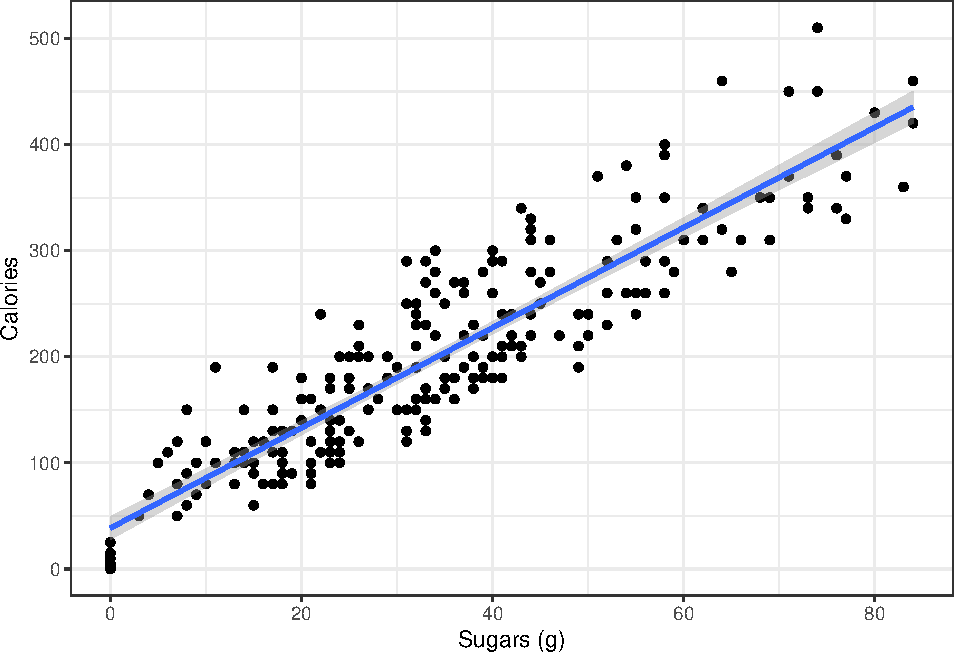
\includegraphics{rladies_dissertation_files/figure-latex/calsugsPlot-1} 

}

\caption{Calories by sugars}\label{fig:calsugsPlot}
\end{figure}

\hypertarget{cross-referencing-figures-and-tables}{%
\section{Cross referencing figures and tables}\label{cross-referencing-figures-and-tables}}

You can cross-reference figures and tables. This is a bit more complicated, but the benefit is that you don't have to remember which figure/table was in which position (especially helpful if you are adding/removing figs/tables during editing phase). You simply refer to the figure by its chunk label.

Figure \ref{fig:figlabel} is shown here.

\begin{figure}
\centering
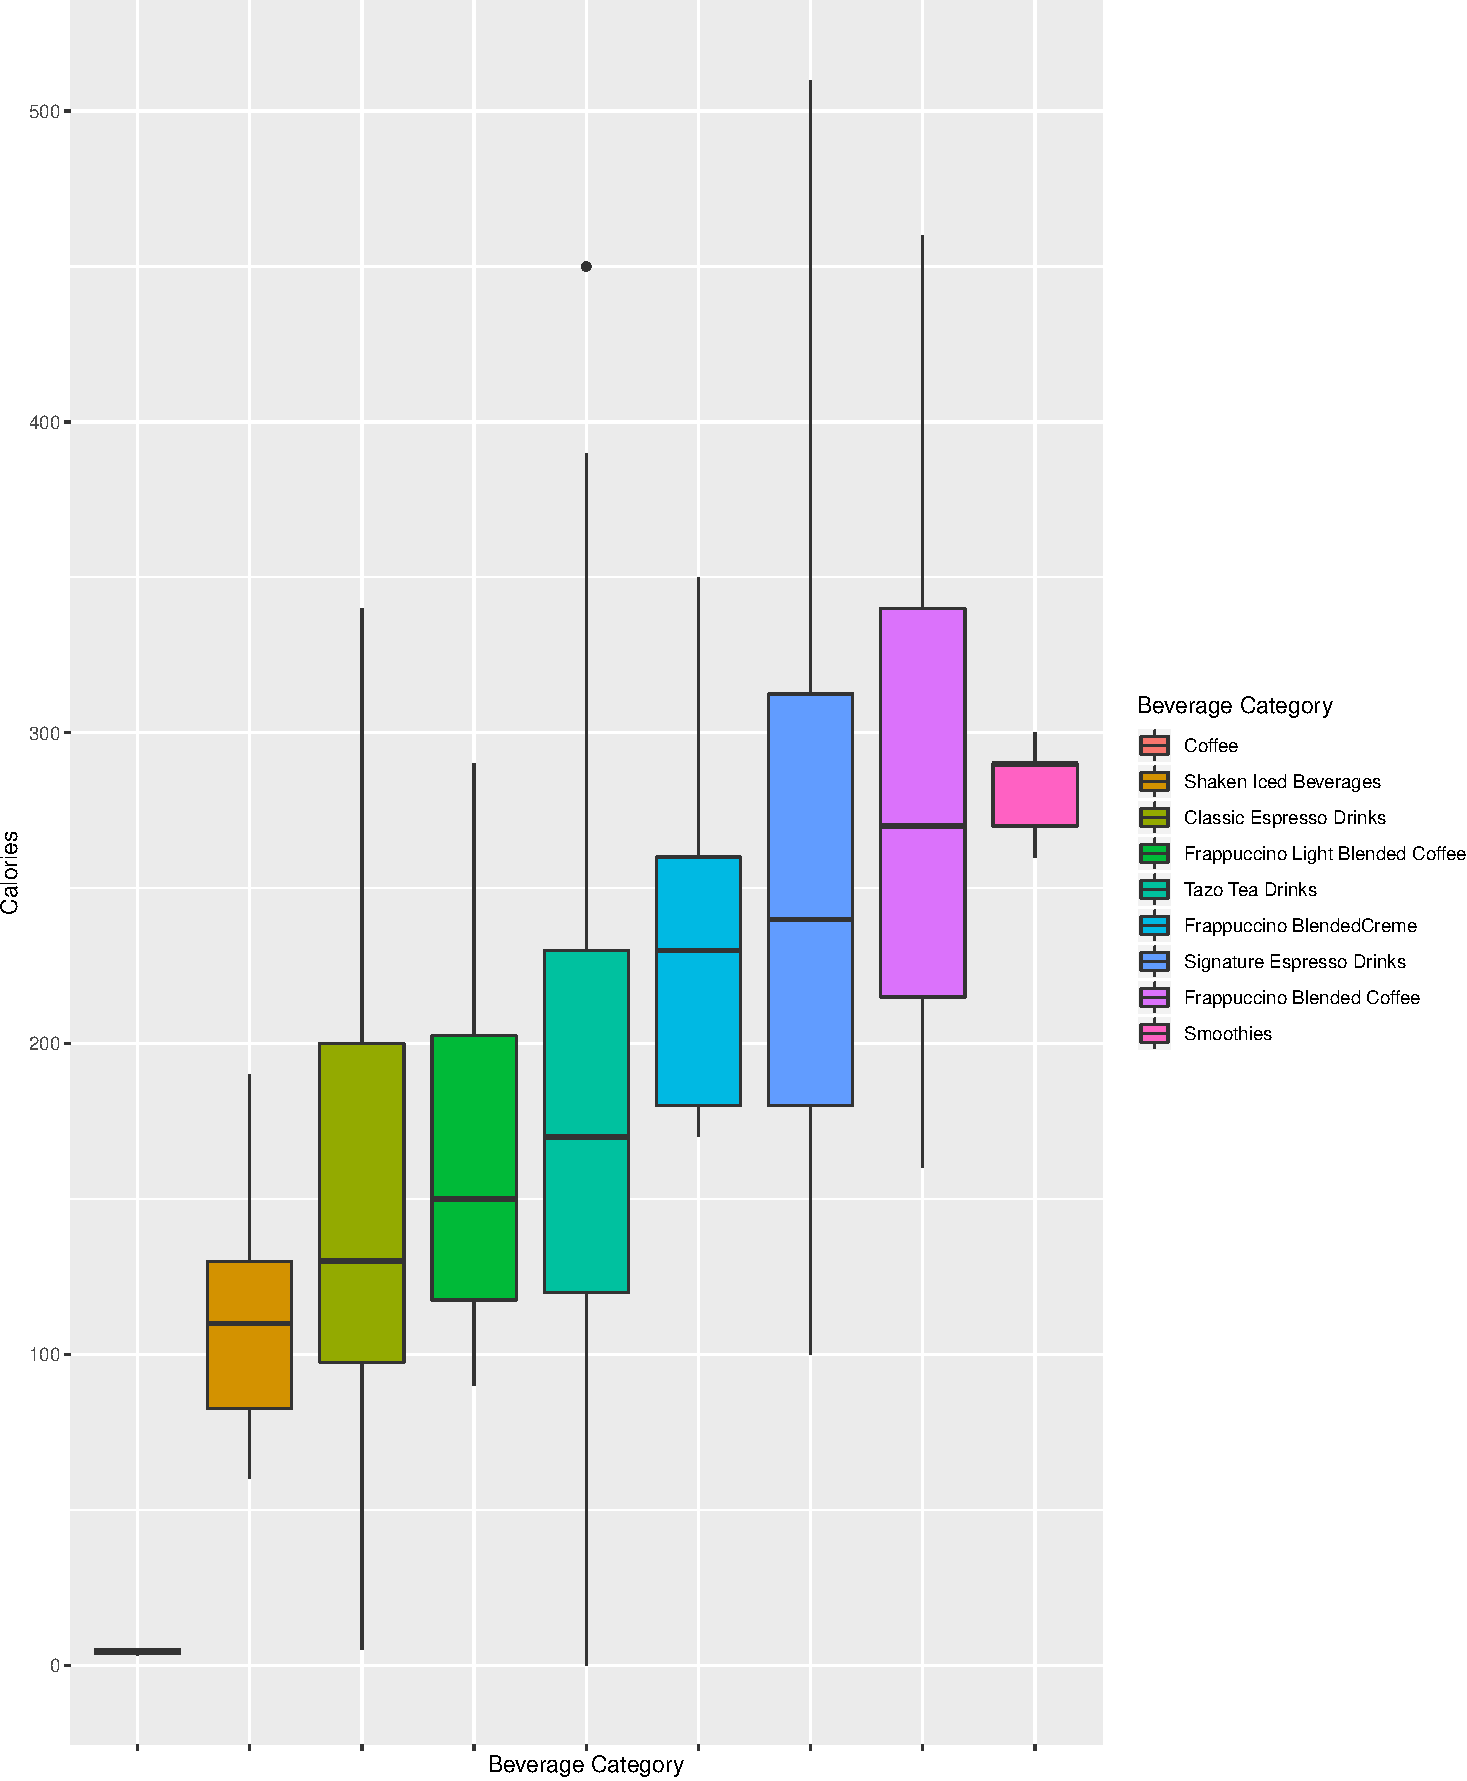
\includegraphics{rladies_dissertation_files/figure-latex/figlabel-1.pdf}
\caption{\label{fig:figlabel}A nice figure caption}
\end{figure}

See Table \ref{tab:calsugs-tab}.

\begin{table}[t]

\caption{\label{tab:calsugs-tab}Calories and sugars for each beverage.}
\centering
\begin{tabular}{lrr}
\toprule
Beverage\_category & cals & sug\\
\midrule
Classic Espresso Drinks & 144.91 & 17.6\\
Coffee & 4.25 & 0.0\\
Frappuccino Blended Coffee & 276.94 & 57.1\\
Frappuccino BlendedCreme & 233.08 & 48.5\\
Frappuccino Light Blended Coffee & 162.50 & 32.4\\
\addlinespace
Shaken Iced Beverages & 114.44 & 26.0\\
Signature Espresso Drinks & 250.00 & 38.6\\
Smoothies & 282.22 & 36.8\\
Tazo Tea Drinks & 177.31 & 30.3\\
\bottomrule
\end{tabular}
\end{table}

We can also just redo the plot

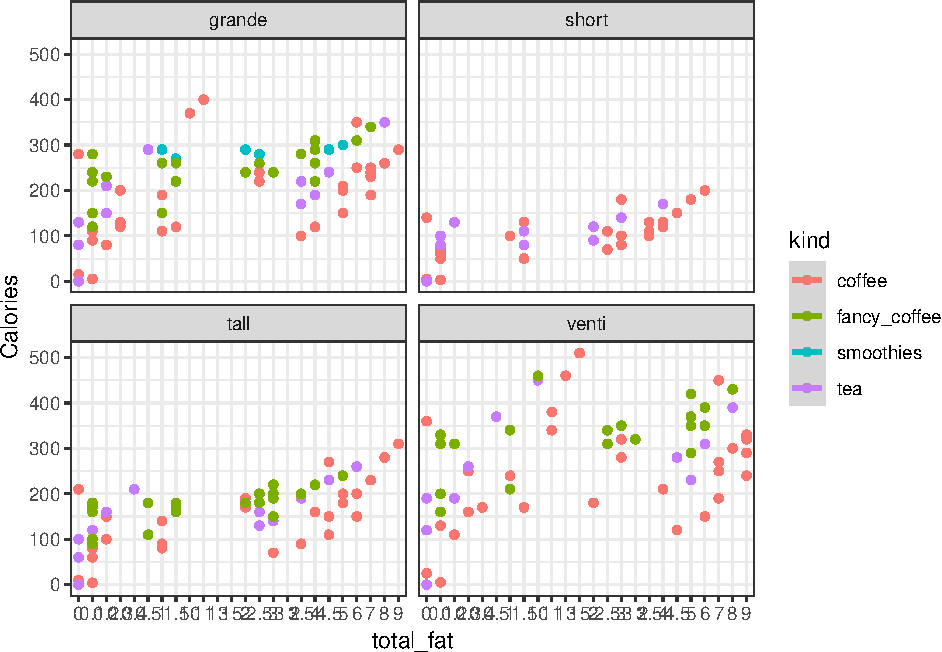
\includegraphics{rladies_dissertation_files/figure-latex/fatPlot-1.pdf}

\hypertarget{using-inline-r-code-to-refer-to-values-in-tables}{%
\subsection{Using inline R code to refer to values in tables}\label{using-inline-r-code-to-refer-to-values-in-tables}}

Here I will include a little extra embedded R code to clean up our model results, but I won't include this code to be shown. In the next paragraph, I'll refer directly to the contents of my model output using in-line R code. For this, we don't use embedded chunks, but rather the syntax `~r someCodeHere `. See the next paragraph in the results.Rmd file for an example.

Sugars demonstrated a significant main effect on the calorie content of starbucks beverages
(estimate = 4.721,
\(t\) = 33.311,
\(p\) = 0).

Notice that our small \(p-value\) shows up as 0, when it really should show up as \textless0.001. I'm going to include another chunk that cleans up the p-value column. Caution: This code is pretty wordy.

Now I'll refer to the same p-value as before, using almost the same inline R code as I did previously. One main difference now, though, is that we've converted the contents of the table to character variables (i.e., they're no longer numeric). We did our rounding in the code above, so I no longer have to round in the inline code.

As previously stated, sugars demonstrated a significant main effect on the calorie content of starbucks beverages
(estimate = 4.721,
\(t\) = 33.311,
\(p\) = \textless0.001).

\hypertarget{printing-a-table}{%
\subsection{Printing a table}\label{printing-a-table}}

Here I will reference a table.

\begin{table}[t]

\caption{\label{tab:mod1Coefs}This is the caption for my model coefficients table.}
\centering
\begin{tabular}{l|l|l|l|l}
\hline
  & Estimate & Std. Error & t value & Pr(>|t|)\\
\hline
(Intercept) & 38.518 & 5.464 & 7.049 & <0.001\\
\hline
sugars & 4.721 & 0.142 & 33.311 & <0.001\\
\hline
\end{tabular}
\end{table}

\textbf{Other stuff}

\begin{itemize}
\tightlist
\item
  How do we change the row names?
\item
  if p \textless{} 0.001, can we write it out that way?
\end{itemize}

\hypertarget{you-can-save-plots}{%
\section{You can save plots}\label{you-can-save-plots}}

Some journals require that you upload figures and tables separately. In this case, it may not make sense to have them print to the document output. The following code will allow you to save an image (default is the working directory) but it won't be included in the document.

\begin{Shaded}
\begin{Highlighting}[]
\KeywordTok{jpeg}\NormalTok{(}\StringTok{"images/pressure.jpg"}\NormalTok{)}
\KeywordTok{plot}\NormalTok{(pressure)}
\KeywordTok{dev.off}\NormalTok{()}
\end{Highlighting}
\end{Shaded}

\begin{verbatim}
## pdf 
##   2
\end{verbatim}

You could, for example, make a subdirectory called ``\texttt{figures}'', and include that in the path.

\hypertarget{conclusions}{%
\chapter{Conclusions}\label{conclusions}}

\hypertarget{another-results-section}{%
\section{Another results section}\label{another-results-section}}

\hypertarget{references}{%
\chapter*{References}\label{references}}
\addcontentsline{toc}{chapter}{References}

\hypertarget{refs}{}
\leavevmode\hypertarget{ref-thompson2004}{}%
Thompson, Craig J, and Zeynep Arsel. 2004. ``The Starbucks Brandscape and Consumers'(anticorporate) Experiences of Glocalization.'' \emph{Journal of Consumer Research} 31 (3): 631--42.

\backmatter
\end{document}
